\documentclass[10pt,a4paper]{article}
\usepackage[utf8]{inputenc}
\usepackage[german]{babel}
\usepackage[T1]{fontenc}
\usepackage{amsmath}
\usepackage{amsfonts}
\usepackage{amssymb}
\usepackage{amsthm}
\usepackage[gen]{eurosym}
\usepackage{graphicx}
\usepackage{paralist}
\usepackage[head=75pt,left=2cm,right=1cm,top=3.8cm,bottom=2cm]{geometry}
\author{Hannes Benne}

\usepackage[code=Code39,X=.4mm,ratio=1.25,H=0.5cm]{makebarcode}

%Definition von Kopf und Fußzeile mit fancyhrd
\usepackage{fancyhdr} 
\pagestyle{fancy}
\fancyhf{}
\rhead{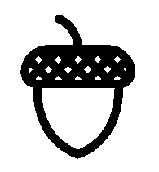
\includegraphics[width=1. cm]{img/logo.png}}
\chead{\textbf{\large{Umsatzauswertung \the\year} \\  \small{Food Squirrel GmbH} } }
\lhead{ Autor \\ Hannes Benne}
\cfoot{Seite \thepage}



\begin{document}
\section*{Jahresverlauf}
Die Food Squirrel GmbH verzeichnete im Jahr \the\year{} einen Umsatz von \VAR{Gesamtumsatz} \euro{}. Der Umsatzstärkste Monat war dabei war der \VAR{Maxmonat} mit einem Umsatz von \VAR{Maxumsatz} \euro{} und der Umsatzschwächste Monat war der \VAR{Minmonat} mit einem Umsatz von \VAR{Minumsatz} \euro.
\begin{figure}[h]
\centering
    \includegraphics[width=1.\textwidth]{img/Jahresumsatz.png}
\caption{Umsatz im Jahresverlauf} 
\end{figure}

\section*{Größte Kunden}
Den größten Umsatz erzielten wir dieses Jahr mit den folgenden Kunden:
\begin{enumerate}
\item \VAR{Kunde1} mit einem Umsatz von \VAR{Umsatz1} \euro,
\item \VAR{Kunde2} mit einem Umsatz von \VAR{Umsatz2} \euro,
\item \VAR{Kunde3} mit einem Umsatz von \VAR{Umsatz3} \euro.
\end{enumerate}
\newpage

\begin{figure}[h]
\centering
    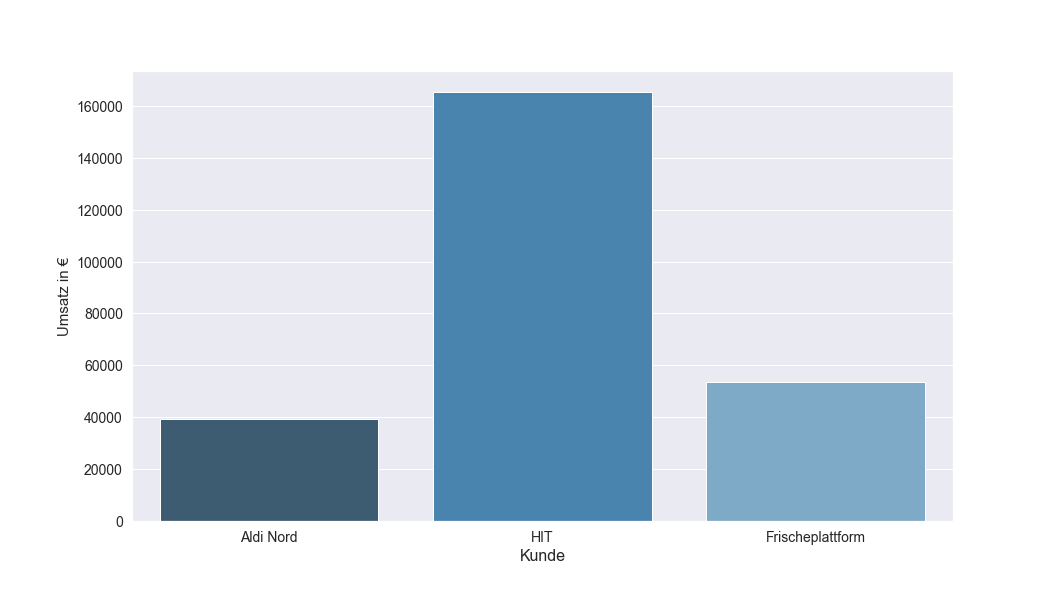
\includegraphics[width=1\textwidth]{img/top_kunden.png}
\caption{Top 3 Kunden} 
\end{figure}

\section*{Top und Flop Produkte}
Am meisten Umsatz brachte das Produkt \VAR{Topprodukt}: \VAR{Topumsatz} \euro. Den geringsten Umsatz brachte das Produkt \VAR{Flopprodukt}: \VAR{Flopumsatz} \euro.

\begin{figure}[h]
\centering
    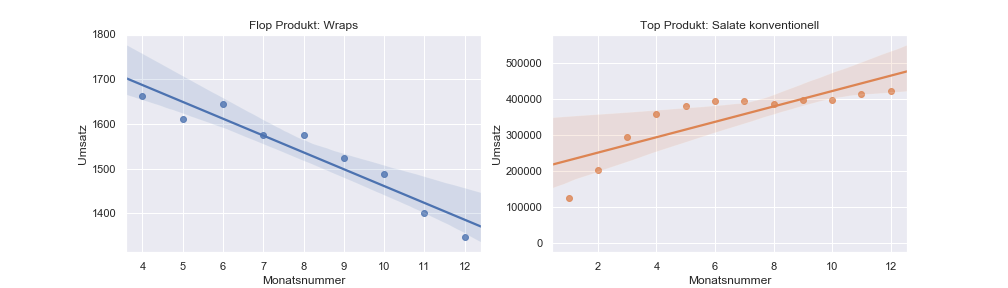
\includegraphics[width=1\textwidth]{img/flopundtop.png}
\caption{Trend für Umsatzschwächstes - und stärkstes Produkt} 
\end{figure}

\end{document}